%----------------------------------------------------------------------------------------
%    PACKAGES AND THEMES
%----------------------------------------------------------------------------------------

\documentclass[aspectratio=169,xcolor=dvipsnames]{beamer}
% \setbeameroption{show notes} %TODO: Thomas a enlever avant la presentation
\usetheme{SimplePlus}

\useoutertheme{miniframes}  % Adds horizontal navigation dots at the top for subsections

\usecolortheme{} 

\setbeamercolor{block title}{bg=structure,fg=white}  % Navy blue background for block titles
\setbeamercolor{block body}{bg=structure!10,fg=black}  % Light navy tint for block body

\definecolor{darkwine}{RGB}{128,0,32}  % Dark red wine
\newenvironment{errorblock}[1]{%
\begingroup%
\setbeamercolor{block title}{bg=darkwine,fg=white}%
\setbeamercolor{block body}{bg=structure!05,fg=black}%  % Very close to white background
\begin{block}{#1}%
}{\end{block}\endgroup}

\usepackage{comment}
\usepackage{hyperref}
\usepackage{graphicx} % Allows including images
\usepackage{booktabs} % Allows the use of \toprule, \midrule and \bottomrule in tables
\usepackage{array} % Allows >{\centering\arraybackslash} in tabular
\usepackage[utf8]{inputenc} % Handle Unicode characters
\usepackage[T1]{fontenc} % Better font encoding
\usepackage{amsmath,amssymb} % Math symbols
\usepackage{algorithm}
\usepackage{algpseudocode}
\usepackage[backend=biber,style=authoryear,maxcitenames=1]{biblatex}
\addbibresource{refs.bib}

% Define hyphenation command
\newcommand{\hyp}{-}

% Define real numbers symbol
\newcommand{\R}{\mathbb{R}}

%----------------------------------------------------------------------------------------
%    TITLE PAGE
%----------------------------------------------------------------------------------------

\title{Diffusion Generative Flow Samplers: Improving Learning Signals Through Partial Trajectory Optimization (ICLR 2024)}

\subtitle{Dinghuai Zhang*, Ricky T. Q. Chen, Cheng-Hao Liu, Aaron Courville \& Yoshua Bengio}
\author{Thomas Mousseau} 

% \institute
% {
%     Department of Computer Science and Information Engineering \\
%     National Taiwan University % Your institution for the title page
% }
\date{\today} % Date, can be changed to a custom date

%----------------------------------------------------------------------------------------
%    PRESENTATION SLIDES
%----------------------------------------------------------------------------------------

\begin{document}

\begin{frame}
    % Print the title page as the first slide
    \vspace*{-2cm}
    \titlepage
\end{frame}

\begin{frame}{Overview}
    % Throughout your presentation, if you choose to use \section{} and \subsection{} commands, these will automatically be printed on this slide as an overview of your presentation
    \tableofcontents
\end{frame}

%------------------------------------------------

\section{Introduction and Motivation}

\subsection{Problem Statement}

\begin{frame}[t]{Generative Modeling}
\scriptsize
\begin{block}{Task}
    Sample from a complex (high-dimensional and multimodal) distribution $D$.
\end{block}

$D$ can be given under the form of:

\begin{columns}[t]
\begin{column}{0.48\textwidth}
\begin{itemize}\itemsep2pt
    \item A dataset of samples $\{x_i\}_{i=1}^N \sim D$ (e.g., images, text, audio)
    \begin{figure}
        \centering
        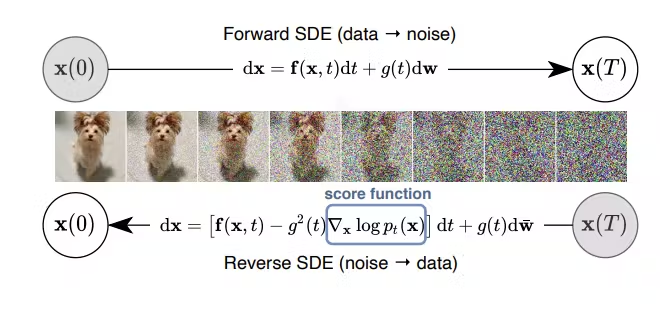
\includegraphics[width=0.9\textwidth]{figures/score_diffusion.png}
    \end{figure}
\end{itemize}
\end{column}
\begin{column}{0.48\textwidth}
\begin{itemize}\itemsep2pt
    \item An unnormalized density $\mu(x)$ where $D$ has density $\pi(x) \propto \mu(x)$ (e.g., 
    energy-based models, physics/chemistry)
    \begin{figure}
        \centering
        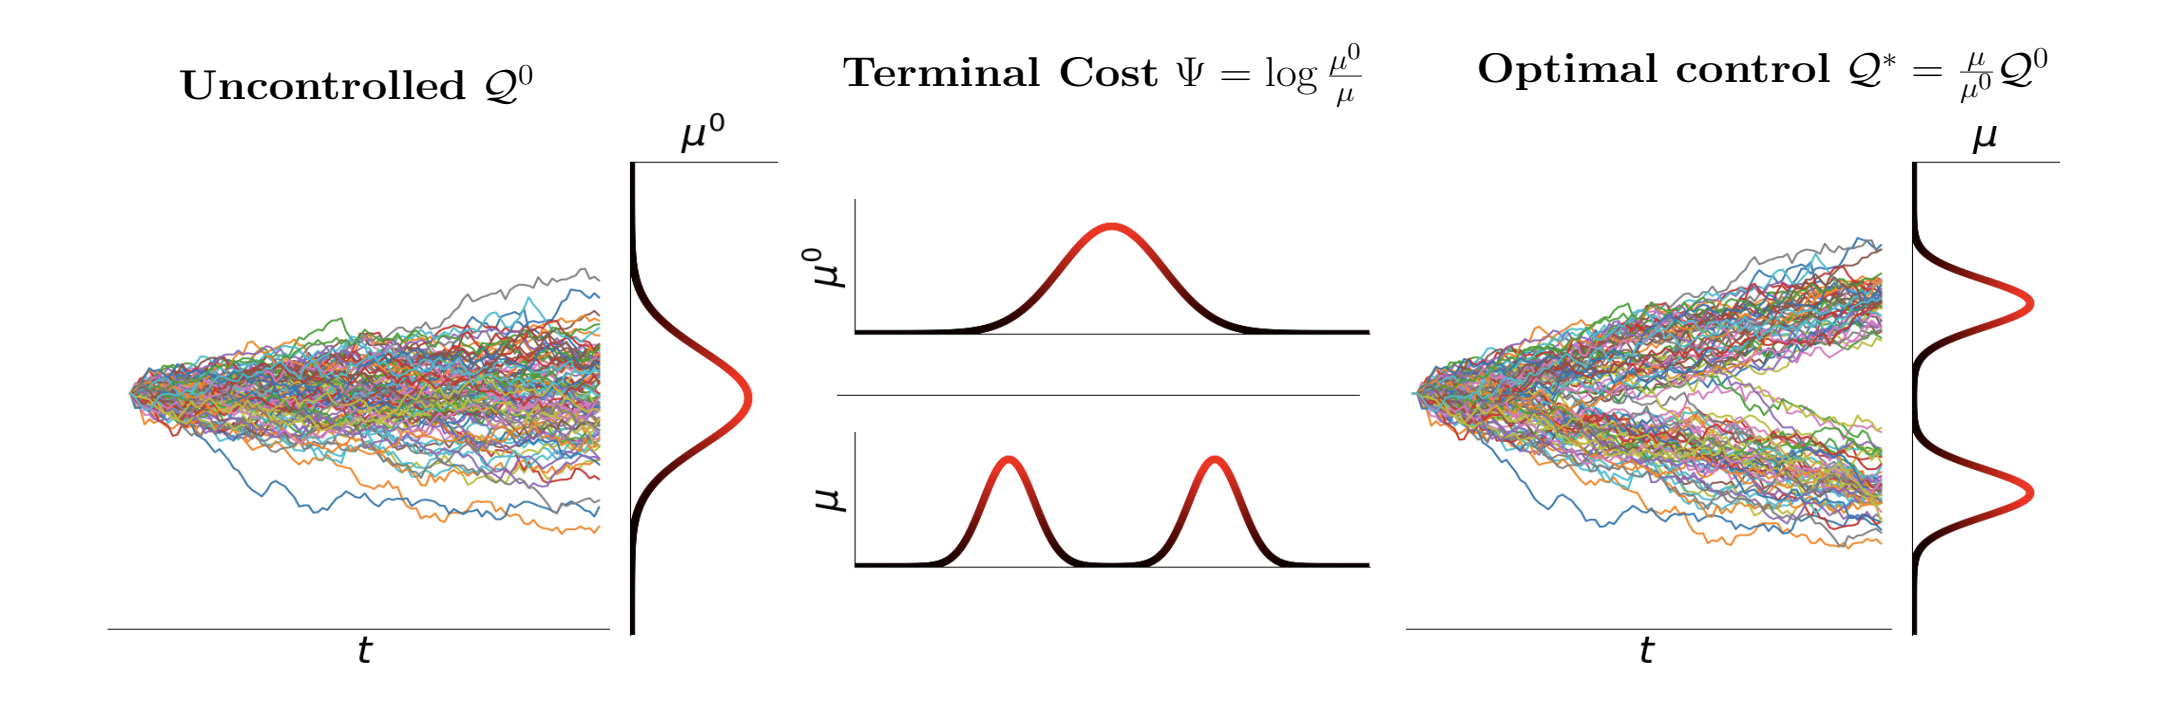
\includegraphics[width=0.9\textwidth]{figures/unconctrolled.png}
    \end{figure}
\end{itemize}
\end{column}
\end{columns}

\end{frame}

\begin{frame}[t]{Sampling from Unnormalized Densities}
\footnotesize
\textbf{Context.} Sample from a $D$-dimensional target with unnormalized density $\mu(x)$ where $\mathbb R^D \to \mathbb R$.
\[
\pi(x)=\frac{\mu(x)}{Z},\qquad Z=\int_{\mathbb R^D}\mu(x)\,dx\ \text{(unknown)}.
\]
We assume we can evaluate $\mu(x)$, but we have no samples from $\pi$ and do not know $Z$.

\vspace{0.1cm}

\medskip
\textbf{Goal.} We seek a \emph{sampler} (similar to MCMC/VI) that produces calibrated samples and, ideally, estimates $Z$ \emph{without} any dataset from $\pi$.

\vspace{0.3cm}

\begin{block}{\scriptsize Chemistry (molecule conformers).} \scriptsize 
    Molecules admit many 3D conformations scored by an energy $E(x)$ (lower is better). We set $\mu(x)=\exp(-E(x))$ so larger $\mu$ means more desirable. Because many chemical properties are unknown or costly, a well-calibrated sampler draws conformers in proportion to $\mu$, yielding high-quality and diverse candidates for ranking, ensemble estimates, and realistic screening than chasing a single best pose.

\end{block}

\end{frame}



\subsection{Stochastic Optimal Control}
\begin{frame}[t]{Controlled and Reference Processes}

\scriptsize

\vspace{-0.2cm}

\begin{block}{\scriptsize Goal.} Learn $f_\theta$ so that the terminal marginal $Q(x_N)$ matches $\mu(x)$ and be proportional to $\pi(x)$ (no data, $Z$ unknown).
\end{block}

\medskip

\begin{columns}[t]
\begin{column}{0.48\textwidth}
\textbf{Controlled forward transition (learned drift).}
\[
P_F(x_{n+1}\mid x_n)\;=\;\mathcal N\!\big(x_{n+1};\;x_n + h\,f_\theta(x_n,n),\;h\sigma^2 I\big)
\]
\textbf{Controlled process and marginals.}
\[
Q(x_{0:N})\;=\;p^{\text{ref}}_0(x_0)\;\prod_{n=0}^{N-1} P_F(x_{n+1}\mid x_n)
\]

\[
p_n(x) = \int Q(x_{0:N})\,dx_{0:n-1}dx_{n+1:N}, \;\text{no closed form.}
\]

\end{column}
\begin{column}{0.48\textwidth}
\textbf{Uncontrolled/Reference forward transition.}
\[
P_F^{\text{ref}}(x_{n+1}\mid x_n)\;=\;\mathcal N\!\big(x_{n+1};\;x_n,\;h\sigma^2 I\big)
\]
\textbf{Uncontrolled/Reference process and marginals.}
\[
Q^{\text{ref}}(x_{0:N})\;=\;p^{\text{ref}}_0(x_0)\;\prod_{n=0}^{N-1} P_F^{\text{ref}}(x_{n+1}\mid x_n),
\]

\[
p^{\text{ref}}_n(x) = \mathcal{N}\left( x; x_0, \Sigma_0 + n h \sigma^2 I \right), \;\text{is closed form.}
\]
\end{column}
\end{columns}

\note{Why closed form for uncontrolled but not controlled? The uncontrolled reference process has no drift, so each transition is a simple Gaussian convolution, leading to Gaussian marginals with closed-form means and variances $(e.g., p^{ref}_n(x) = N(x; mu_0, cov_0 + n h \sigma^2 I))$. The controlled process includes a learned drift $f(x_n, n)$, which makes transitions non-Gaussian and dependent on $f$, preventing a closed-form marginal expression without solving the integral numerically or via simulation.


\textcolor{red}{je dois refaire cette slide, on ne voit meme comment xn est sample (par rapport a la SDE) et aussi d'ou sort sigma mu et la closed form expliquer et c'est une convolution de gaussienne}}

\end{frame}

\begin{frame}{Closed Form of Reference Marginal}
\footnotesize

\textbf{Uncontrolled Sampling.}
\[
x_N = x_0 + \sqrt{h} \sigma \sum_{k=0}^{N-1} \varepsilon \quad \varepsilon \sim \mathcal{N}(0, I) \quad \text{since we are using Brownian motion}.
\]

\textbf{Gaussian Form (Reparametrization Trick).}
\[
x_N \sim \mathcal{N}(x_0, \Sigma_0 + N h \sigma^2 I) \quad \text{where } \Sigma_0 \text{ is the initial covariance.}
\]

\textbf{Probability Density Function of Terminal Marginal Distribution.}
\[
p^{\text{ref}}_N(x_N) = \frac{1}{(2\pi)^{D/2} |\Sigma_0 + N h \sigma^2 I|^{1/2}} \exp\left( -\frac{1}{2} (x_N - x_0)^\top (\Sigma_0 + N h \sigma^2 I)^{-1} (x_N - x_0) \right).
\]

\end{frame}


\begin{frame}{Guiding the Controlled Process}
\footnotesize

\begin{block}{\footnotesize Adding Terminal Tilt to the Uncontrolled $Q^{\text{ref}}$ Process to Create the Target Process $P$}

\[
P(\tau) = Q^{\text{ref}}(x_{0:N-1} | x_N) \cdot \pi(x_N) = Q^{\text{ref}}(\tau) \cdot \frac{\pi(x_N)}{p_N^{\text{ref}}(x_N)} \propto Q^{\text{ref}}(\tau) \cdot \frac{\mu(x_N)}{p_N^{\text{ref}}(x_N)}.
\]
    
\end{block}

% \textbf{Goal.} We want the terminal marginal of the controlled process to match the target distribution:

% \[
% P(x_N) = \pi(x_N), \quad \text{but to reach } x_N, \text{ we will need a trajectory that goes from } x_0 \text{ to } x_N
% \]

\medskip


\[
P(x_N) = \int_{\text{subtrajectories}} \underbrace{Q^{\text{ref}}(x_{0:N-1} | x_N) \, dx_{0:N-1} \cdot p_N^{\text{ref}}(x_N)}_{Q^{\text{ref}}(x_{0:N})} \cdot \frac{\pi(x_N)}{p_N^{\text{ref}}(x_N)} = \pi(x_N).
\]

% \medskip

% By adding a terminal tilt, the target process $P(\tau)$ biases every step of the trajectory towards regions where $\pi(x_N)$ is high:




\end{frame}


\begin{frame}[t]{Path space KL objective}
\scriptsize


\textbf{Target path measure via terminal reweighting.}
\[
P(x_{0:N})\propto\ Q^{\text{ref}}(x_{0:N})\,\frac{\mu(x_N)}{p^{\text{ref}}_N(x_N)}
\qquad\Longrightarrow\qquad P(x_N)\propto\mu(x_N).
\]

\textbf{KL decomposition using Girsanov theorem (path space).}
\[
\mathrm{KL}(Q\|P)
=\mathbb E_{Q}\!\left[\log\frac{Q}{P}\right]
=\mathbb E_{Q}\!\left[\log\frac{Q}{Q^{\text{ref}}}\right]
+\mathbb E_{Q}\!\left[\log\frac{p^{\text{ref}}_N(x_N)}{\mu(x_N)}\right] + \log Z.
\]


\medskip
\textbf{Running cost.}
\[
\mathbb E_{Q}\!\left[\log\frac{Q}{Q^{\text{ref}}}\right]
=\mathbb E_Q\!\big[\sum_{n=0}^{N-1}\frac{h}{2\sigma^2}\,\|f_\theta(x_n,n)\|^2\big].
\]

\textbf{Terminal cost.}
\[
\mathbb E_{Q}\!\left[\log\frac{p^{\text{ref}}_N(x_N)}{\mu(x_N)}\right]
=\mathbb E_Q\!\big[\log p^{\text{ref}}_N(x_N)-\log \mu(x_N)\big].
\]

\end{frame}


\section{Method}

\subsection{Solving Credit Assignment Problem}

\begin{frame}[t]{Credit Assignment Problem in SOC objective}
\footnotesize

\vspace{0.8cm}

\begin{errorblock}{SOC Discrete-time objective}
\[
\min_{f_\theta}\ \mathbb E_Q\!\Big[\underbrace{\sum_{n=0}^{N-1}\tfrac{h}{2\sigma^2}\|f_\theta(x_n,n)\|^2}_{\text{Running cost}}\;+\;\underbrace{\log p^{\text{ref}}_N(x_N)-\log \mu(x_N)}_{\text{Terminal cost}}\Big]
\]

This objective is used on the seminar paper \emph{Path Integral Sampler: Diffusion-based Sampling for Unnormalized Densities} \cite{zhang2022} which presented the sampling from unnormalized densities as a stochastic optimal control problem.

\end{errorblock}

% \textbf{Explanation.} The SOC objective provides feedback signal only at the terminal step, making credit assignment difficult via backpropagation through time. This causes high-variance gradients, weak feedback for early actions, poor mode discovery, and inefficient optimization of the drift $f$ without intermediate signals.

\end{frame}

\begin{frame}[t]{SOC as a GFlowNet}
\footnotesize

\textbf{Comparison Table: GFlowNet vs. SOC Framework}

\begin{table}[h]
\centering
\footnotesize
\begin{tabular}{@{}lcc@{}}
\toprule
\textbf{Concept} & \textbf{GFlowNet} & \textbf{SOC} \\
\midrule
\textbf{Forward Process} & Trajectory sampling on DAG & Controlled diffusion path \\
\textbf{Forward Transition Probability} & $P_F(s' | s)$ & $P_F(x_{n+1} | x_n) = \mathcal{N}(x_{n+1}; x_n + h f_\theta(x_n), h\sigma^2 I)$ \\
\textbf{Backward Transition Probability} & $P_B(s | s')$ & $P_B^{\text{ref}}(x_n | x_{n+1})$ (known) \\
\textbf{Reward Function} & $R(x)$ (unnormalized) & $\mu(x)$ (unnormalized density) \\
\textbf{Terminal Marginal Distribution} & $P_T(x) \propto R(x)$ & $Q(x_N) \propto \mu(x_N)$ \\
\textbf{Flow State} & Flow $F(s)$ at states & Learned flow $F_n(x)$ \\
\bottomrule
\end{tabular}
\end{table}

\textbf{Insight.} Since SOC can be viewed as a GFlowNet, we can apply GFlowNet tools (detailed balance loss or subtrajectory balance) to solve the credit assignment problem.

\note{make a mental note to comeback to professor hernandez comment on Tristan's Deleu presentation when someone asked: "The if GFlowNets are just Reinfrocement Learning, then why keep doing research on this framework?" Professor Hernandez reponded by proving the felxibility of GFN, he said that it was en entery point between RL, Diffusion models, Energy-based models and in this case we prove that it can also be used in Stochastic Optimal Control problems.}

\end{frame}

% \begin{frame}[t]{Insight in solving credit assignment problem}
% \footnotesize

% \textbf{What if we could know or approximate the target distribution at any step $n$?}

% \[
% P(x_0, \dots, x_N) := Q^{\text{ref}}(x_0, \dots, x_N) \frac{\pi(x_N)}{p^{\text{ref}}_N(x_N)}.
% \]

% Using the reference bridge decomposition:
% \[
% Q^{\text{ref}}(x_{0:N}) = Q^{\text{ref}}(x_{0:N-1} | x_N) \, p_N^{\text{ref}}(x_N),
% \qquad p_N^{\text{ref}}(x_N) = \int Q^{\text{ref}}(x_{0:N}) \, dx_{0:N-1}.
% \]

% \[
% P(x_{0:N}) = \pi(x_N) \prod_{n=0}^{N-1} P_B(x_n | x_{n+1}),
% \]

% \small
% \textbf{Key fact.} Because the terminal reweighting only touches $x_N$, the backward kernel of $P$ at intermediate steps equals the \emph{reference} backward kernel (a Gaussian bridge for our reference).\\
% \textbf{Hard part.} The intermediate marginal $p_n(x_n)$ has no closed form in general $\Rightarrow$ we amortize it via a learned $F_n(x_n)$.

% Unfortunately, although we know the form of $P_B(\cdot|\cdot)$, for general target distribution there is generally no known analytical expression for it. As a result, we propose to use a deep neural network $F_n(\cdot; \theta)$ with parameter $\theta$ as a “helper” to approximate the unnormalized density of the $n$-th step target $p_n(\cdot)$.
% \end{frame}


\subsection{GFlowNet}

\begin{frame}[t]{Adressing Credit Assignment via Target Process}
\footnotesize

\begin{errorblock}{SOC Discrete-time objective}
\[
\min_{f_\theta}\ \mathbb E_Q\!\Big[{\sum_{n=0}^{N-1}\tfrac{h}{2\sigma^2}\|f_\theta(x_n,n)\|^2}\;+\;{\log p^{\text{ref}}_N(x_N)-\log \mu(x_N)}\Big]
\]

\end{errorblock}

% \begin{errorblock}{Target process necessitates terminal reweighting...}
%     \[
% P(x_{0:N}) \propto Q^{\text{ref}}(x_{0:N}) \frac{\mu(x_N)}{p^{\text{ref}}_N(x_N)} \implies P(x_N) \propto \mu(x_N).
% \]
% \end{errorblock}

\begin{block}{Could we write the target process differently to allow intermediate supervision?}

    \textbf{Conditional Form.} Since the reweighting only affects the terminal state, the joint can be written as:
\[
P(x_{0:N}) = \pi(x_N) \prod_{n=0}^{N-1} Q_B^{\text{ref}}(x_n | x_{n+1}),
\]
where $Q_B^{\text{ref}}(\cdot | \cdot)$ is the backward transition probability (derived from the target joint). This is tractable because $Q_B^{\text{ref}}$ is known.

\end{block}

\end{frame}

% \begin{frame}[t]{Rewriting the Target Process with Marginal}
% \tiny

% \textbf{Rewriting the Joint Using Marginal Densities.} The backward factorization of the target process is:
% \[
% P(x_{0:N}) = \pi(x_N) \prod_{n=0}^{N-1} P_B^{\text{ref}}(x_n | x_{n+1}).
% \]

% To express it in terms of the marginal densities $p_n(x_n)$, note that the marginal at step $n$ is obtained by integrating out the future states $x_{n+1:N}$ from the joint:
% \[
% p_n(x_n) = \int P(x_{0:N}) \, dx_{0:n-1} \, dx_{n+1:N} = \int \pi(x_N) \prod_{l=n}^{N-1} P_B^{\text{ref}}(x_l | x_{l+1}) \, dx_{n+1:N} \propto \int \mu(x_N) \prod_{l=n}^{N-1} P_B^{\text{ref}}(x_l | x_{l+1}) \, dx_{n+1:N}.\]
% This shows that $p_n(x_n)$ is the "unnormalized" density at step $n$, propagated backward from the terminal $\pi(x_N)$ via the backward transitions.

% \textbf{What $p_n(x_n)$ Represents.} 
% \begin{itemize}\itemsep2pt
%   \item $p_N(x_N) = \pi(x_N)$: The terminal marginal, which is the normalized target density we want to match (proportional to $\mu(x_N)$).
%   \item For $n < N$, $p_n(x_n)$ is the marginal density at step $n$ under the target process $P$. It represents how likely the state $x_n$ is at time $n$, given that the trajectory will eventually reach a terminal state distributed as $\pi(x_N)$. In other words, it's the distribution of $x_n$ marginalized over all possible future paths that lead to $\pi(x_N)$.
%   \item Intuitively, $p_n(x_n)$ encodes the "value" or importance of being at $x_n$ at step $n$, as it accounts for the probability of reaching high-$\mu$ terminals from there. This is why approximating $p_n(x_n)$ allows training with partial trajectories starting from step $n$.
% \end{itemize}

% \textbf{Why This Helps in Writing the Target Process.} The joint $P(x_{0:N})$ can be thought of as a chain where each $p_n(x_n)$ summarizes the "progress" toward the terminal, but the backward form directly ties it to $\pi(x_N)$. By learning $F_n \approx p_n$, we can reconstruct or approximate the joint without computing the full integral, enabling efficient partial-trajectory optimization.

% \end{frame}

\begin{frame}[t]{Rewriting the Target Process with Marginal}
\scriptsize

\textbf{If We Had Access to $p_n(x_n)$} we could write the partial joint which would allow training on subtrajectories and thus have better credit assignment:
\[
P(x_{0:n}) = p_n(x_n) \prod_{k=0}^{n-1} Q^\text{ref}_B(x_k | x_{k+1}),
\]

\textbf{But There's No Closed Form for $p_n(x_n)$.} To calculate $p_n(x_n)$, we would need to compute the integral:
\[
p_n(x_n) = \int_{\mathbb{R}^{(N-n)D}} \pi(x_N) \prod_{k=n}^{N-1} Q^\text{ref}_B(x_k | x_{k+1}) \, dx_{n+1:N}.
\]

\[
p_n(x_n) \propto \int_{\mathbb{R}^{(N-n)D}} \mu(x_N) \prod_{k=n}^{N-1} Q^{\text{ref}}_B(x_k | x_{k+1}) \, dx_{n+1:N}.
\]

\vspace{-0.2cm}

\begin{errorblock}{\scriptsize Why is $p_n(x_n)$ hard to compute?}
\scriptsize To calculate this this high-dimensional integral (from $n$ to $N$ over $D$ dimensions), we would need a solution like Monte Carlo quadratures which would be infeasible in practice, especially since training requires computing it repeatedly for subtrajectories as intermediate signals.

\end{errorblock}

% \textbf{Why is $p_n(x_n)$ hard to compute?} The integral represents summing over all possible future paths from $x_n$ to the terminal $x_N$, weighting each by the terminal density $\pi(x_N)$. This high-dimensional integration (over $(N-n)\times D$ dimensions) has no analytical solution for general $\mu(x_N)$. Numerically approximating it via quadratures or Monte Carlo is computationally expensive, especially since training requires computing it repeatedly for subtrajectories as intermediate signals (replacing the single terminal signal), making it impractical.

\note{ne pas oublier de parler des MC quadrature method pour approximer l'integral mais c'est couteux en temps de calcul et pas scalable du tout}

\end{frame}

% \begin{frame}[t]{PartialTrajectory Balance with Learned Flow}
% \footnotesize

% \textbf{Proposed Amortized Approach.} Train $F_n(\cdot; \phi)$, a neural network, to satisfy the following constraint for all partial trajectories $x_{n:N}$:
% \[
% F_n(x_n; \phi) \prod_{k=n}^{N-1} P_F(x_{k+1} | x_k; \theta) = \mu(x_N) \prod_{k=n}^{N-1} P_B(x_k | x_{k+1}).
% \]

% \textbf{Details.}
% \begin{itemize}\itemsep2pt
%   \item $P_F$ (forward policy) and $F_n$ are parameterized by deep neural networks, with parameters $\theta$ and $\phi$ respectively.
%   \item We can view $F_n$ as an approximation to the unknown marginal $p_n(x_n)$ thus an amortized way to estimate the intractable integral.
%   \item We use only $\mu(\cdot)$ (no $Z$), so the unknown normalization is absorbed into $F_n$.
%   \item Very similar to a Value Function in RL, estimating future expected rewards (here, future density mass).
% \end{itemize}
% \end{frame}

\begin{frame}[t]{Detailed and SubTB Balance with Learned Flow}
\footnotesize


\vspace{0.5cm}

\begin{errorblock}{Detailed Balance Condition with Learned Flow} 
\[
F_n(x_n; \phi) P_F(x_{n+1} | x_n; \theta) = F_{n+1}(x_{n+1}; \phi) P_B(x_n | x_{n+1}).
\]

\end{errorblock}

\medskip


\begin{block}{Subtrajectory Balance Loss for Partial Trajectories}

    \[
\ell_{\text{SubTB}}(x_{m:n}; \theta, \phi) = \left( \log \frac{F_m(x_m; \phi) \prod_{k=m}^{n-1} P_F(x_{k+1} | x_k; \theta)}{F_n(x_n; \phi) \prod_{k=m}^{n-1} P_B(x_k | x_{k+1})} \right)^2
\]

Using a mix of different subtrajectory lengths $(m,n)$ allows better credit assignment thus more stable training of both the forward policy and the learned flow.
    
\end{block}

\note{a voir si je voudrais pas mettre une schema sur l'une des 3 derniers slides pour faire un recap de scrap la SOC objective, now we build DB loss with learned flow to solve credit assignment problem}

\end{frame}

\begin{frame}[t]{Overall Training Objective}
\scriptsize

\vspace{0.1cm}

\begin{block}{\scriptsize Recall SubTB Loss}
\scriptsize
\[
\ell_{\text{SubTB}}(x_{m:n}; \theta, \phi) = \left( \log \frac{F_m(x_m; \phi) \prod_{k=m}^{n-1} P_F(x_{k+1} | x_k; \theta)}{F_n(x_n; \phi) \prod_{k=m}^{n-1} P_B(x_k | x_{k+1})} \right)^2
\]
\end{block}

\begin{errorblock}{\scriptsize Diffusion Generative Flow Sampler (DGFS) Loss}
    \scriptsize
\[
L(\tau; \theta; \phi) = \frac{\sum_{0 \leq m < n \leq N} \lambda^{n-m} \ell_{\text{SubTB}}(x_{m:n})}{\sum_{0 \leq m < n \leq N} \lambda^{n-m}}, \quad \tau = (x_0, \dots, x_N)
\]

\textbf{This combines signals from all subtrajectory lengths, reducing variance and improving credit assignment}
\begin{itemize}\itemsep2pt
  \item $\tau$: Full trajectory $(x_0, \dots, x_N)$.
  \item $\lambda$: $(0, 1]$ to weight shorter subtrajectories more since they have lower variance.
  \item The denominator stabilizes the loss scale across different trajectory lengths.
\end{itemize}

\end{errorblock}

\end{frame}


\begin{frame}[t,fragile]{}
\footnotesize  

\vspace{-0.35cm}

\begin{algorithm}[H]
    \footnotesize
\caption{DGFS Training}
\label{alg:dgfs}
\begin{algorithmic}[1]
\Require $\mu(\cdot)$, $\bar{\sigma}$, $N$, $\lambda$, $B$, $\eta$
\State Init $\theta=(\theta_f,\phi)$
\Repeat
    \State Sample trajectories:
    \For{$b=1$ to $B$}
        \State $\tau^{(b)}=(x^{(b)}_0,\ldots,x^{(b)}_N)$ under $x_{n+1}=x_n+h f_{\theta}(x_n,n)+\sqrt{h}\bar{\sigma}\varepsilon_n$, $\varepsilon_n\sim\mathcal N(0,I)$
    \EndFor
    \State Build subtrajectories: $\mathcal S(\tau^{(b)})$ of $(m,n)$ with $0\le m<n\le N$
    \State Compute SubTB loss:
    \begin{equation*}
\mathcal L(\tau^{(b)};\theta)=\frac{\sum_{(m,n)\in\mathcal S(\tau^{(b)})}\lambda^{n-m}\left[\log\frac{F_\phi(x_m)\prod_{l=m}^{n-1} P_F(x_{l+1}\mid x_l;\theta_f)}{F_\phi(x_n)\prod_{l=m}^{n-1} P_B^{\mathrm{ref}}(x_l\mid x_{l+1})}\right]^2}{\sum_{(m,n)\in\mathcal S(\tau^{(b)})}\lambda^{n-m}}
    \end{equation*}
    \State $g \leftarrow \nabla_{\theta}\frac{1}{B}\sum_{b=1}^B \mathcal L(\tau^{(b)};\theta)$
    \State $\theta \leftarrow \mathrm{Adam}(\theta, g, \eta)$
\Until{convergence}
\end{algorithmic}
\end{algorithm}
\end{frame}


%------------------------------------------------
\section{Results}

\subsection{Comparaing with Prior Methods}

\begin{frame}[t]{Reduction of Gradient Variance}
\footnotesize

\vspace{-0.75cm}
\begin{columns}[t]
\begin{column}{0.35\textwidth}
\begin{figure}
    \centering
    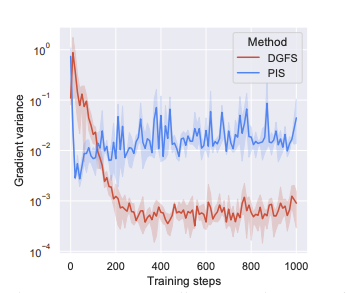
\includegraphics[width=\textwidth]{figures/grad_variance.png}
    \caption{Gradient variance comparison between DGFS and PIS. DGFS shows significantly lower variance, leading to more stable training.}
\end{figure}
\end{column}
\begin{column}{0.35\textwidth}
\begin{figure}
    \centering
    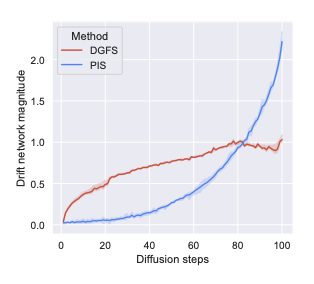
\includegraphics[width=\textwidth]{figures/drift.png}
    \caption{Drift network magnitude of DGFS and PIS.}
\end{figure}
\end{column}
\end{columns}

\end{frame}


\begin{frame}[t]{Partition Function Estimation}
\footnotesize

\vspace{1.2cm}

\begin{block}{Partition Function Estimation}
\[
\log \sum_{\tau}^\mathrm{B} \exp(\log(P(\tau)) - \log(Q(\tau))) - \log \mathrm{B} \leq \log Z, \quad \tau \sim Q(\cdot; \theta).
\]

The equation computes a lower bound on $\log Z$ via importance sampling: it samples trajectories $\tau$ from $Q$, reweights them by $\log(P(\tau)/Q(\tau))$, and uses log-sum-exp to approximate $\log$ of the normalized weight sum, which underestimates $\log Z$ due to Jensen's inequality.

\end{block}

\end{frame}

\begin{frame}[t]{Partition Function Estimation Results}
\footnotesize

\begin{figure}
    \centering
    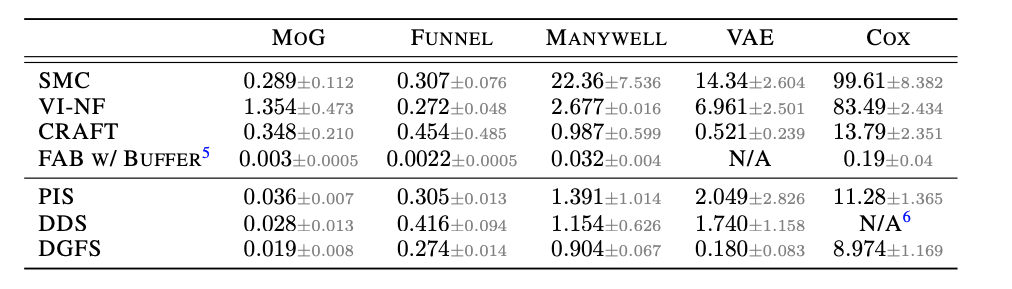
\includegraphics[width=1.025\textwidth]{figures/partition_fnct.png}
    \caption{The lower the better, DGFS achieves the lowest bias in estimating the partition function across various benchmarks except when compared to FAB w/ BUFFER.}
\end{figure}

\end{frame}

\begin{frame}[t]{Mode coverage results}

\begin{columns}[t]
\begin{column}{0.48\textwidth}
\begin{figure}
    \centering
    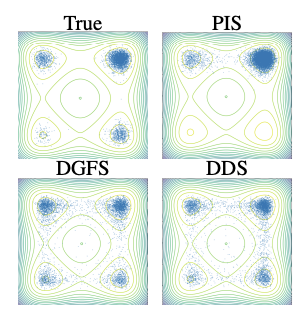
\includegraphics[width=0.5\textwidth]{figures/mode.png}
    \caption{Manywell plots. DGFS and DDS but not PIS recover all modes}
\end{figure}
\end{column}
\begin{column}{0.48\textwidth}
\begin{figure}
    \centering
    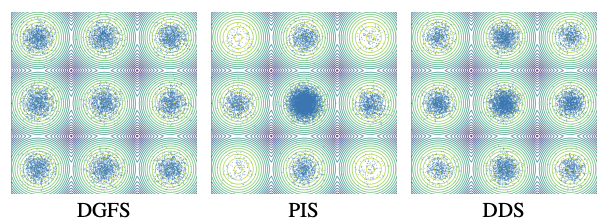
\includegraphics[width=0.9\textwidth]{figures/MoG.png}
    \caption{MoG visualization of DGFS and other diffusion-based samplers shows that DGFS could capture the diverse modes well. The contours display the landscape of the target density}
\end{figure}
\end{column}
\end{columns}
    
\end{frame}

%------------------------------------------------
\section{Conclusion}

\subsection{Strengths and Weaknesses}

\begin{frame}{Strengths of DGFS}
\footnotesize

\begin{block}{Strengths}
\begin{itemize}\itemsep2pt
    \item \textbf{Many intermediate signals} lead to better credit assignment, thus improving convergence speed, training stability, and reducing gradient variance.
    \item \textbf{Better credit assignment} also led to better mode discovery and thus helped reducing the lower bound on many of the benchmarks compared to other path space samplers (PIS \cite{zhang2021path} and DDS \cite{vargas2023denoising}).
    \item Proposed a new dynamic between \textbf{Stochastic Optimal Control}, \textbf{Sampling from an unnormalized density}, and \textbf{GFlowNet}.
    \item Kept \textbf{convergence guarantees} from PIS seminar work.
\end{itemize}
\end{block}

\end{frame}

\begin{frame}{Weaknesses of DGFS}
\footnotesize

\begin{errorblock}{Weaknesses / Limitations}
\begin{itemize}\itemsep1pt
    \item \textbf{Hyperparameter sensitivity}: A great part of the Appendix was dedicated to ablation studies, thus showing that the hyperparameters do vary a lot depending on the experiments.
    \item \textbf{New framework introduces a second neural network}, which increases the training difficulty of this algorithm.
    \item Even if it showed the best results among the path samplers in the benchmark, it was still magnitudes behind the FAB algorithm and \textbf{showed a lot of difficulties in the intermediate to hard level experiments}, thus increasing my doubts regarding the usage of this algorithm in a true complex highly dimensional setting for real world applications.
\end{itemize}
\end{errorblock}

\end{frame}

\begin{frame}{Future Work}
\footnotesize


\begin{itemize}\itemsep2pt
  \item \textbf{Rare event sampler:} By changing the framework, we would be able to emphasize rare event samples given an unnormalized distribution. By showing good mode discovery, we could train this sampler to retrieve many low-likelihood situations in order to prepare critical systems or safety systems in order to prepare them for all possibilities, not only the most likely.
  \item \textbf{Latent space path:} We have seen many diffusion models papers taking the approach of diffusing on a latent space instead of the sample space (Stable Diffusion and DALL-E). Would this technique be as effective in a latent path space as it is in a latent sample space?
  \item \textbf{Introducing more tricks from RL:} We could see that one of the really good performing samplers was FAB w/ BUFFER and they even talked slightly about off-policy in DGFS. It would be very interesting to implement replay buffer, off-policy exploration strategies, and other tricks which RL relies on to improve its performances.
\end{itemize}

\end{frame}

\subsection{Q\&A}

\begin{frame}{Questions and hopefully answers :)}
    \centering
    \Huge Questions!
\end{frame}

\begin{frame}[allowframebreaks]{References}
\footnotesize
\printbibliography
\end{frame}


\end{document}